

\section{Beispiel}

\begin{frame}{Aufgabe}
	\begin{itemize}
		\item Webserver für Most Useless Machine Ever!
	\end{itemize}
	\begin{center}
		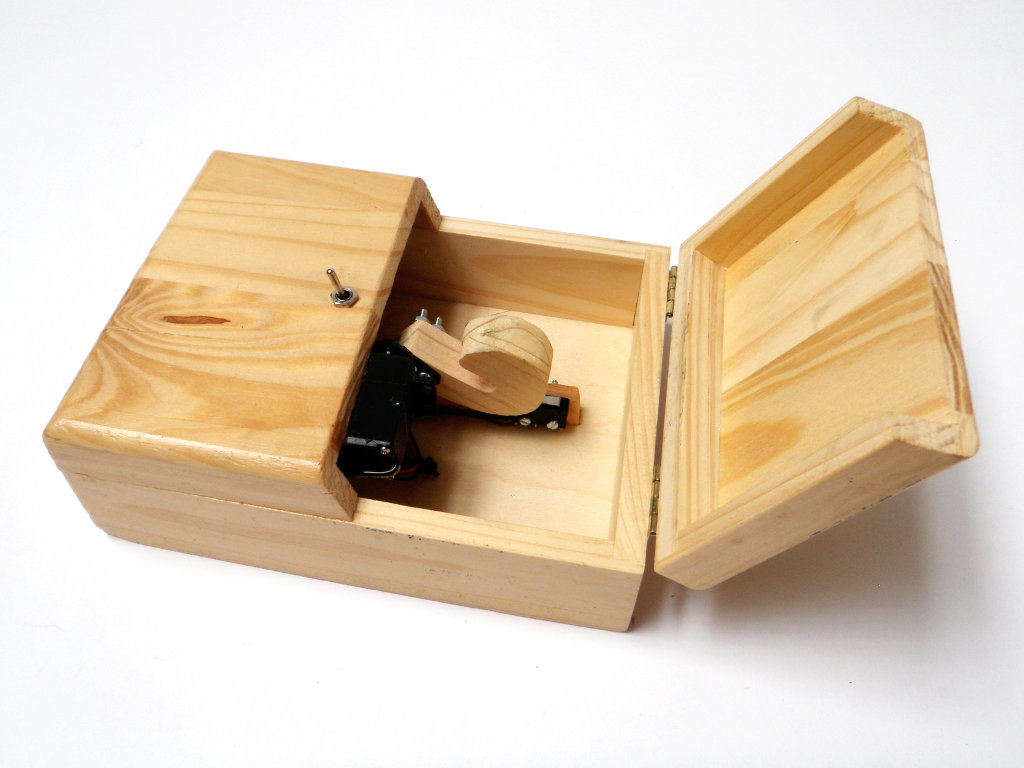
\includegraphics[width=0.75\textwidth]{res/mume.jpg}
		\cite{mumePic}
	\end{center}
\end{frame}

\begin{frame}{System}
	\begin{itemize}
		\item uC oder GNU/Linux?
		\item uC wie Arduino
		\begin{itemize}
			\item Echtzeit
			\item niedrige System-Komplexität
			\item keine Infrastruktur
		\end{itemize}
		\item GNU/Linux
		\begin{itemize}
			\item Treiber
			\item Protokolle
			\item Memory und Prozess Management
			\item hohe System-Komplexität
		\end{itemize}
	\end{itemize}
\end{frame}

\begin{frame}{Hardware}
	\begin{itemize}
		\item Eval-/Bastelboards (Raspi, BeagleBone)
		\item Consumer Hardware (Router, Media-Center, \ldots)
		\item Profesionelle Boards
		\item[$\rightarrow$] BeagleBone Green
		\begin{itemize}
			\item Netzwerk
			\item USB
			\item Yocto Supported
			\item viele Anshlüsse
			\item USB Powered
			\item kein Display Anschluss
			\item bereits Erfahrung
		\end{itemize}
	\end{itemize}
\end{frame}

\begin{frame}{GNU/Linux Distribution}
	\begin{itemize}
		\item Yocto\cite{whyYocto} \footnote{Tools und Rezepte um eigene GNU/Linux Distribution zu bauen}
		\begin{itemize}
			\item git repository mit Konfiguration des gesamten System
			\item Patches einzelner Pakete
			\item Optimierungen für spezifische Hardware
			\item volle Kontrolle
		\end{itemize}
		\item off-the-shelf (Debian, Arch, Gentoo, Ubuntu)
		\begin{itemize}
			\item weite Verbreitung; bekannt
			\item Updates werden von anderen bereitgestellt
			\item erlaubt Lizenz Verteilung?
		\end{itemize}
	\end{itemize}
\end{frame}

\begin{frame}[fragile]{Yocto Image}
	\begin{multicols}{2}
		\begin{lstlisting}[title=mume-dev-image.bb,frame=single,language=bitbake]
LICENSE = "MIT"

inherit core-image
inherit populate_sdk_qt5

IMAGE_INSTALL = " \
  packagegroup-core-boot \
  @\ldots@-core-ssh-openssh \
  packagegroup-mume-common \
  packagegroup-dev-mume \
  \
  mupro-start \
"

IMAGE_FEATURES += " \
  package-management \
  debug-tweaks \
"
		\end{lstlisting}
		\begin{lstlisting}[title=packagegroup-dev-mume.bb, frame=single, numbers=right, language=bitbake]
SUMMARY = "developer tools for MUME"
LICENSE = "MIT"

inherit packagegroup

RDEPENDS_${PN} = "\
  bash \
  devmem2 \
  e2fsprogs \
  htop \
  nginx \
  openssh-sftp \
  perf \
  qtbase \
  strace \
  time \
  @\ldots@
		\end{lstlisting}
	\end{multicols}
\end{frame}

\begin{frame}[fragile]{Yocto Image bauen}
	\begin{lstlisting}[frame=single,language=bash]
$ bitbake mume-dev-image
	\end{lstlisting}
	\begin{table}
		\caption{tmp/deploy/images/beaglebone/}
		\begin{tabular}{ll}
			\hline MLO & stage 1 loader \\ 
			\hline u-boot.img & stage 2 loader \\ 
			\hline uEnv.txt & u-boot Konfiguration \\ 
			\hline zImage & Kernel \\ 
			\hline zImage-bonegreen-mume.dtb & Device Tree \\ 
			\hline mume-dev-image-beaglebone.tar.bz2 & rootfs \\ 
			\hline 
		\end{tabular} 
	\end{table}
\end{frame}

\begin{frame}{rootfs}
	\begin{itemize}
		\item userspace
		\item ev. Kernel \& Device Tree
		\item nicht bootloader
	\end{itemize}
\end{frame}

\begin{frame}{Device Tree}
	\begin{itemize}
		\item meiste Hardware ist nicht Plug and Play
		\item wir müssen Linux mitteilen, wo welche Hardware liegt
		\item Device Tree listet auf, wo sich welche Hardware befindet
		\item Linux lädt Treiber anhand Infos in Device Tree
	\end{itemize}
	\begin{itemize}
		\item Struktur ähnlich wie XML
		\item gegliedert nach BUS
		\item beschreibt welche Hardware angeschlossen ist
		\item Hierarchisch aufgebaut wie Hardware (SOC, Modul, Gerät, System)
	\end{itemize}
	Beispiel
\end{frame}

\begin{frame}{Boot Process \cite{OMAPBootloaderOverview}}
	\begin{tabular}{|l|l|l|}
		\hline typ & name & funktion \\ 
		\hline system startup & ROM Code & minimal hardware initialisierung \\ 
		& & in boot devices nach image suchen \\
		& & stage 1 loader ins ram laden und ausführen \\
		
		\hline stage 1 loader & x-loader (u-boot) & pin muxing \\ 
		& & clock und memory initialisieren \\
		& & stage 2 loader ins ram laden und ausführen \\
		
		\hline stage 2 loader & u-boot & platform initialisierung (USB, Netzwerk, \ldots) \\
		& & boot menu / Kommandozeile anzeigen \\
		& & Kernel und Device-Tree ins ram laden und ausführen \\
		
		\hline kernel & Linux & Treiber für Hardware laden \\ 
		& & root file system mounten \\
		& & init process starten \\
		
		\hline init & Systemd & Abhängigkeiten zwischen Services auflösen \\ 
		& & Services starten \\
		& & Services überwachen \\
		
		\hline 
	\end{tabular} 
\end{frame}

\begin{frame}[fragile]{SDK bauen}
	\begin{lstlisting}[frame=single,language=bash, breaklines=true]
$ bitbake mume-dev-image -c populate_sdk
$ ls -sh tmp/deploy/sdk/
695M mume-glibc-x86_64-mume-dev-image-cortexa8hf-vfp-neon-toolchain-2.0.sh
	\end{lstlisting}
	\begin{itemize}
		\item Cross-Compiler
		\item Entwicklerpakete (header, \ldots)
		\item root file system (libraries, \ldots)
		\item Paketmanager
	\end{itemize}
\end{frame}

\begin{frame}{Services (Applikation)}
\end{frame}

\begin{frame}{Hardware ansteuern / Treiber}
	\begin{itemize}
		\item wie können wir die Hardware ansteuern?
		\item[$\rightarrow$] Linux Treiber, Frameworks, Infrastructure:
		\begin{itemize}
			\item GPIO
			\item PWM
			\item sysfs
			\item Device-Tree
			\item wait-queue
			\item interrupt
		\end{itemize}
	\end{itemize}
\end{frame}

\begin{frame}{MUME Service}
	\begin{itemize}
		\item wie können wir mit dem Treiber kommunizieren?
		\item[$\rightarrow$] sysfs / D-Bus
		\begin{itemize}
			\item Service der den Treiber weiter abstrahiert
		\end{itemize}
	\end{itemize}
\end{frame}

\begin{frame}{GUI}
	\begin{itemize}
		\item Koennen wir via Browser auf das System zugreifen?
		\item[$\rightarrow$] gui
		\begin{itemize}
			\item nginx
			\item fastcgi
			\item gui
			\item D-Bus
		\end{itemize}
	\end{itemize}
\end{frame}

\begin{frame}{Service Manager}
	\begin{itemize}
		\item Wie starten und managen wir die Services?
		\item[$\rightarrow$] systemd
		\begin{itemize}
			\item service files schreiben
			\item fastcgi
			\item gui
			\item D-Bus
		\end{itemize}
	\end{itemize}
\end{frame}

\begin{frame}{Produktiv Image}
	\begin{itemize}
		\item Wie können wir die Firmware verteilen?
		\item[$\rightarrow$] Yocto
	\end{itemize}
\end{frame}







\begin{frame}{system}
	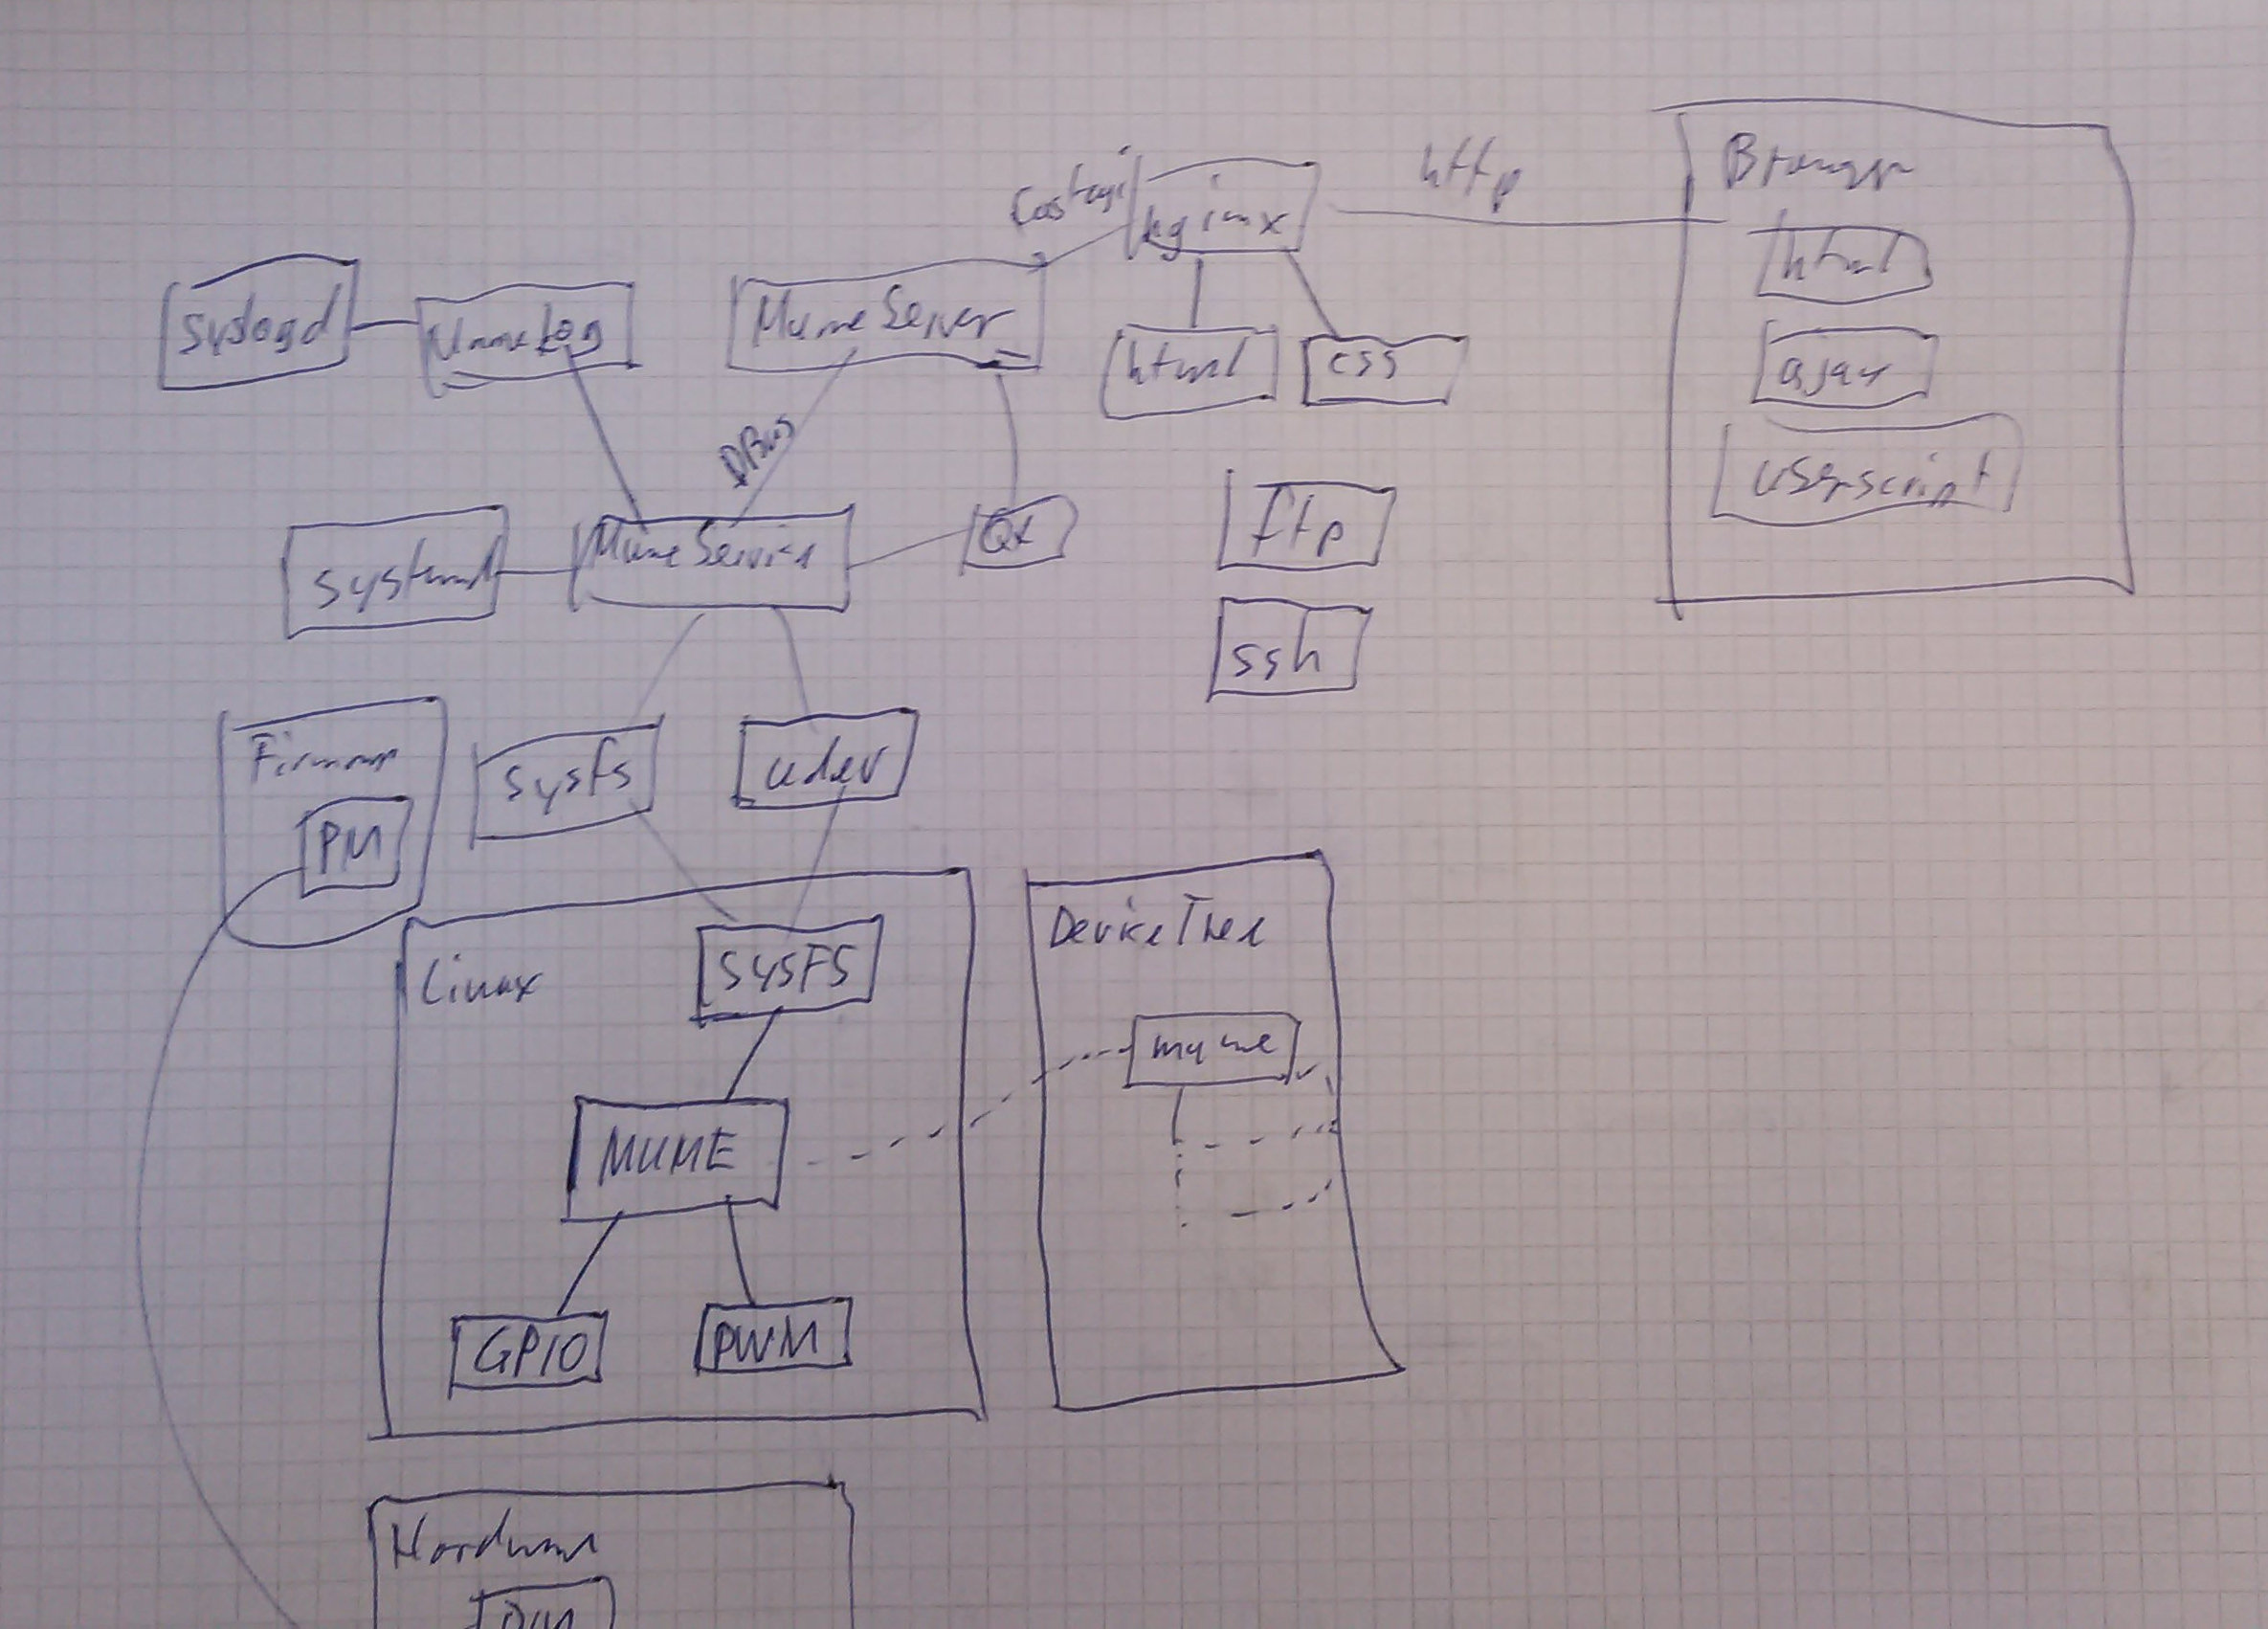
\includegraphics[width=\textwidth]{res/system.jpg}
\end{frame}

\begin{frame}{Linux}
	\begin{itemize}
		\item Sammlung von Subsystemen, abstraktionenen
		\item i2c
		\item spi
		\item iio
		\item fbtft
		\item gpio
		\item led
	\end{itemize}
\end{frame}

\begin{frame}{eigener Treiber}
	Beispiel ``Most Usless Machine Ever''
\end{frame}

\begin{frame}{Applikationen}
	Siehe System
	\begin{itemize}
		\item Embedded System besteht meist aus mehreren Prozessen $\rightarrow$ Microservices
		\item Webserver, Prozessueberwachung, SSH, FTP, UI
		\item gutes IPC system (z.B. kdbus)
		\item eigener Service
		\begin{itemize}
			\item reaktiv, event-getriggert
			\item Qt gut geeignet
			\item andere Frameworks moeglich
			\item auch ohne Framework moeglich
		\end{itemize}
	\end{itemize}
\end{frame}

\begin{frame}{Webserver}
\end{frame}